% This is a Basic Assignment Paper but with like Code and stuff allowed in it, there is also url, hyperlinks from contents included. 

\documentclass[11pt]{article}

% Preamble

\usepackage[margin=1in]{geometry}
\usepackage{amsfonts, amsmath, amssymb, amsthm}
\usepackage{fancyhdr, float, graphicx}
\usepackage[utf8]{inputenc} % Required for inputting international characters
\usepackage[T1]{fontenc} % Output font encoding for international characters
\usepackage{fouriernc} % Use the New Century Schoolbook font
\usepackage[nottoc, notlot, notlof]{tocbibind}
\usepackage{listings}
\usepackage{xcolor}
\usepackage{blindtext}
\usepackage{hyperref}
\definecolor{codepurple}{rgb}{0.58,0,0.82}
\hypersetup{
    colorlinks=true,
    linkcolor=black,
    filecolor=black,      
    urlcolor=codepurple,
    pdfpagemode=FullScreen,
    }

\definecolor{codegreen}{rgb}{0,0.6,0}
\definecolor{codegray}{rgb}{0.5,0.5,0.5}
\definecolor{backcolour}{rgb}{0.95,0.95,0.92}

\lstdefinestyle{mystyle}{
    backgroundcolor=\color{backcolour},   
    commentstyle=\color{codegreen},
    keywordstyle=\color{magenta},
    numberstyle=\tiny\color{codegray},
    stringstyle=\color{codepurple},
    basicstyle=\ttfamily\footnotesize,
    breakatwhitespace=false,         
    breaklines=true,                 
    captionpos=b,                    
    keepspaces=true,                 
    numbers=left,                    
    numbersep=5pt,                  
    showspaces=false,                
    showstringspaces=false,
    showtabs=false,                  
    tabsize=2
}

\lstset{style=mystyle}

% Header and Footer
\pagestyle{fancy}
\fancyhead{}
\fancyfoot{}
\fancyhead[L]{\textit{\Large{Cyber Crime Investigation Manual V1}}}
\fancyhead[R]{\textit{Parth Zarekar}}
\fancyfoot[C]{\thepage}
\renewcommand{\footrulewidth}{1pt}
\newtheorem{thm}{Theorem}
\newtheorem{dfn}[thm]{Definition}


% Other Doc Editing
% \parindent 0ex
%\renewcommand{\baselinestretch}{1.5}

\begin{document}

\begin{titlepage}
    \centering

    %---------------------------NAMES-------------------------------

    \huge\textsc{
        MIT World Peace University
    }\\

    \vspace{0.75\baselineskip} % space after Uni Name

    \LARGE{
        Vulnerability Identification and Penetration Testing\\
        Third Year B. Tech, Semester 6
    }

    \vfill % space after Sub Name

    %--------------------------TITLE-------------------------------

    % \rule{\textwidth}{1.6pt}\vspace*{-\baselineskip}\vspace*{2pt}
    % \rule{\textwidth}{0.6pt}
    \vspace{0.79\baselineskip} % Whitespace above the title



    \huge{\textsc{
            CSI: Cyber Crime Investigation Manual
        }} \\



    \vspace{6\baselineskip} % Whitespace below the title
    % \rule{\textwidth}{0.6pt}\vspace*{-\baselineskip}\vspace*{2.8pt}
    % \rule{\textwidth}{1.6pt}

    \vspace{1\baselineskip} % Whitespace after the title block

    %--------------------------SUBTITLE --------------------------	

    \LARGE\textsc{
        Manual Version 1
    } % Subtitle or further description
    \vfill

    %--------------------------AUTHOR-------------------------------

    Prepared By
    \vspace{0.5\baselineskip} % Whitespace before the editors

    \Large{
        Parth Zarekar \\
    }


    \vspace{0.5\baselineskip} % Whitespace below the editor list
    \today

\end{titlepage}


\tableofcontents
\thispagestyle{empty}
\clearpage

\setcounter{page}{1}



\section{\textbf{Recovery of Hacking Instagram Accounts}}


\section{\textbf{Recovery of Hacked Facebook Accounts}}

\section{\textbf{Telegram Investigation}}
\url{telemetr.io} can be used for Investigation related to telegram channels which were involved inn the crime.
Telemetr helps give a profile of the channel including the real subscriber and the grown of the channel over periodic timeframes.

\begin{figure}[H]
    \centering
    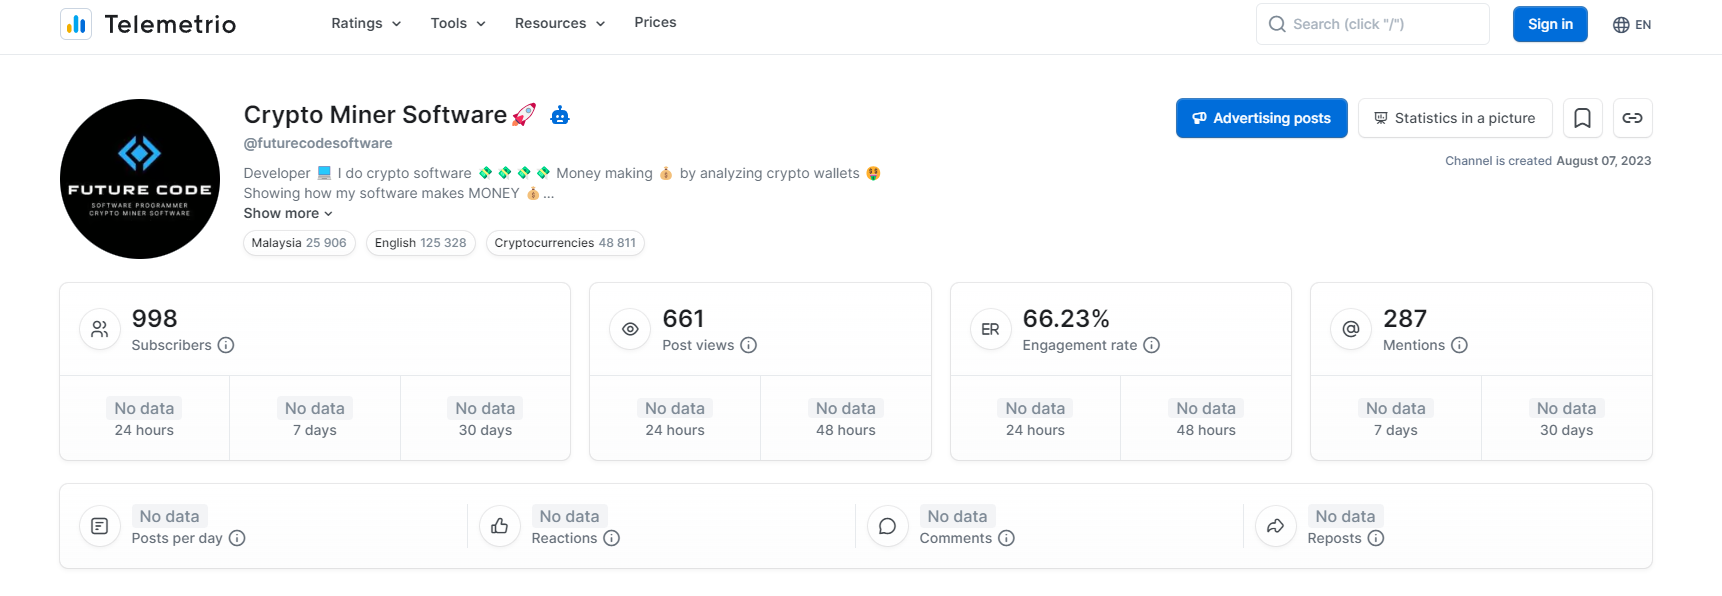
\includegraphics[width=0.8\textwidth]{./imgs/telemetrio2.png}
    \caption{Telemetr.io}
    \label{fig:telemetr}
\end{figure}

\textbf{TOOLS url:} \url{https://telemetr.io/en}

\section{\textbf{Investigation of Fraud Website}}

\subsection{\textbf{Website registration details investigation}}
A WHOIS lookup is a process used in website investigation to gather information about domain registration. This information can be used to identify the owner of the domain, the domain registrar, and the domain’s registration and expiration dates. WHOIS lookups can also provide information about the domain’s name servers, the domain’s status, and the domain’s contact information.
\begin{itemize}
    \item \textbf{Name server:} The DNS (domain name System) servers that are authoritative for the domain
    \item \textbf{Status of the domain:} Whether the domain is active, expired, on hold, etc.
    \item \textbf{ownership Verification:} It helps verify the legitimacy of a website by confirming the details provided byt during the domain registration process.
    \item \textbf{Contact Information:} It provides contact details of the domain owner, which can be useful for reaching out in case of legal or technical issues.
    \item \textbf{Domain History:} By looking at the registration and expiration dates, you can get an idea of how long a website has been in existence.
    \item \textbf{Name Server information:} This can be relevant for understanding the hosting infrastructure of a website.
\end{itemize}

\begin{figure}[H]
    \centering
    \includegraphics[width=0.8\textwidth]{./imgs/whois.png}
    \caption{WHOIS Lookup}
    \label{fig:whois}
\end{figure}

\textbf{TOOLS url:} 
\begin{itemize}
    \item \url{https://whois.domaintools.com/}
    \item \url{https://www.whois.com/}
\end{itemize}

\subsection{\textbf{Website History Investigation}}
\textbf{Wayback Machine} is a digital archive of the World Wide Web and other information on the Internet. It allows the user to go back in time and see what a website looked like in the past. It is a great tool for website investigation as it can help you understand the history of a website, including how it has evolved over time, what content has been added or removed, and how the website has been used by different people. Information gather from the wayback machine are:
\begin{itemize}
    \item \textbf{Archived Versions of the Website:} The primary function of the Wayback Machine is to provide access to historical snapshots of websites. Users can enter a URL and view different version of a webpage captured at various points in time.
    \item \textbf{Website Changes overtime:} By navigating through different snapshots, you can observe how a website has evolved, see design changes, and track the addition or removal of content.
    \item \textbf{Availability Status:} You can determine if a website was accessible and archived on specific dates. This is particularly useful for Investigating the historical Availability of a site. 
\end{itemize}

\begin{figure}[H]
    \centering
    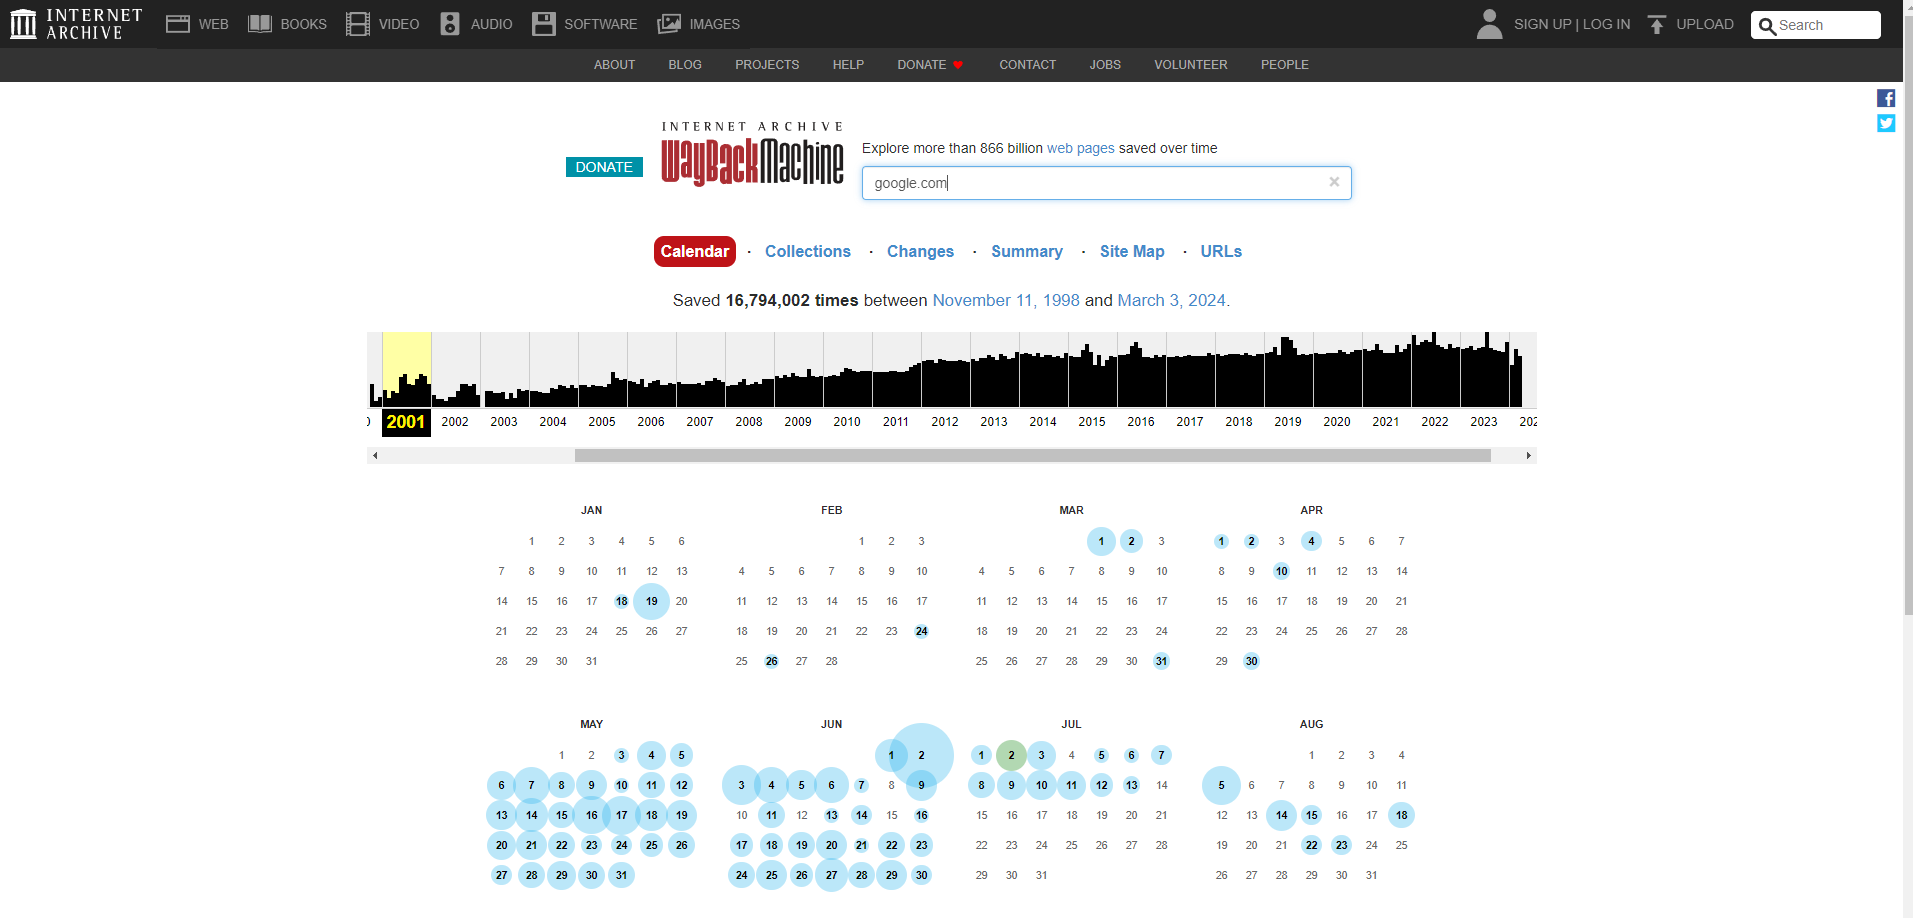
\includegraphics[width=0.8\textwidth]{./imgs/Wayback Machine.png}
    \caption{Wayback Machine}
    \label{fig:wayback}
\end{figure}

\textbf{TOOLS url:}
\begin{itemize}
    \item \url{https://archive.org/web/}
\end{itemize}

\section{\textbf{Investigation For Phishing and Fraudulent websites}}
Scam Advisor is a Valuable online tool for Investigating the legitimacy of websites, particularly those suspected of phishing or fraudulent activities. Users can simply visit the scam Advisor website, input the URL of the website in question, and receive a comprehensive report. The report includes a scam score indicating the risk level, a trust score for evaluating reliability, and details on domain age, popularity, and ownership. Users can delve into server location, user reviews, and contact information to assess the website's credibility. Scam Advisor empowers individuals to make informed decisions about the trustworthiness of websites, contributing to a safer online environment.

\subsection {Step1:} 
Visit the Scam Advisor website and enter the URL of the website you want to investigate.
\url{scamadvisor.com}

\clearpage

\pagebreak


\end{document}